\documentclass[t]{beamer}

\usepackage{amsmath}
\usepackage{pgfplots}
\usepackage{soul}
\usepackage{tikz}

\pgfplotsset{compat=1.9}

\usetheme{metropolis}

\author{Esten H{\o}yland Leonardsen}
\institute[Life Science, UiO]{UiO:Life Science, University of Oslo}
\date{02.11.22}
\title{Introduction to deep learning 1/?}

\titlegraphic{
	\vspace*{6.8cm}
	\centering
    \includegraphics[width=1.5cm]{data/uio.png}
}

\makeatletter
\let\UL\ul
\renewcommand\ul{%
  \let\set@color\beamerorig@set@color
  \let\reset@color\beamerorig@reset@color
  \UL}

\begin{document}

	\def\nodesize{14pt}
	\begin{frame}
		\titlepage
	\end{frame}

	\begin{frame}{Introduction}
		\vfill
		\centering
		\begin{enumerate}
			\item Building an artificial neural network (ANN)
			\item Training the ANN
			\item Transformation to a Convolutional Neural Network (CNN)
		\end{enumerate}
		\vfill
	\end{frame}

	\begin{frame}{Building a neural network: Linear regression}
		\centering
		\vfill
		\begin{tikzpicture}
			\node[] at (-5, 3) {};
			\node[] at (5, -4.5) {};

			\node[] at (0, 0) {$y=ax+b$};
		\end{tikzpicture}
		\vfill
	\end{frame}

	\begin{frame}{Building a neural network: Linear regression}
		\centering
		\vfill
		\begin{tikzpicture}
			\node[] at (-5, 3) {};
			\node[] at (5, -4.5) {};

			\node[] at (0, 0) {$y=ax+b$};

			\draw[] (-2, -1.5) -- (2, -1.5) -- (2, -4) -- (-2, -4) -- (-2, -1.5);

			\draw[very thick, blue!60] (-2, -3.5) -- (2, -1.75);

			\node[anchor=north] at (0, -4.1) {x};
			\node[anchor=south, rotate=90] at (-2.1, -2.75) {y};
		\end{tikzpicture}
		\vfill
	\end{frame}

	\begin{frame}{Building a neural network: Linear regression}
		\centering
		\vfill
		\begin{tikzpicture}
			\node[] at (-5, 3) {};
			\node[] at (5, -4.5) {};

			\node[
				circle,
				draw=black,
				fill=green!20,
				minimum size=\nodesize,
				inner sep=0pt
			] (n) at (0, 1.5) {};
			\node[] (x) at (-1.5, 1.5) {$x$};
			\node[] (b) at (0, 2.5) {$b$};
			\node[] (y) at (1.5, 1.5) {$y$};
			\node[] at (0, 0) {$y=ax+b$};

			\draw[->] (x) -- (n) node [midway, above] {$a$};
			\draw[->] (b) -- (n);
			\draw[->] (n) -- (y);

			\draw[] (-2, -1.5) -- (2, -1.5) -- (2, -4) -- (-2, -4) -- (-2, -1.5);

			\draw[very thick, blue!60] (-2, -3.5) -- (2, -1.75);

			\node[anchor=north] at (0, -4.1) {x};
			\node[anchor=south, rotate=90] at (-2.1, -2.75) {y};
		\end{tikzpicture}
		\vfill
	\end{frame}

	\begin{frame}{Building a neural network: Artificial neuron}
		\centering
		\vfill
		\begin{tikzpicture}
			\node[] at (-5, 3) {};
			\node[] at (5, -4.5) {};

			\node[
				circle,
				draw=black,
				fill=green!20,
				minimum size=\nodesize,
				inner sep=0pt
			] (n) at (0, 1.5) {};
			\node[] (x) at (-1.5, 1.5) {$x$};
			\node[] (b) at (0, 2.5) {$b$};
			\node[] (y) at (1.5, 1.5) {$y$};
			\node[] at (0, 0) {$y=max(0, wx+b)$};

			\draw[->] (x) -- (n) node [midway, above] {$w$};
			\draw[->] (b) -- (n);
			\draw[->] (n) -- (y);

			\draw[] (-2, -1.5) -- (2, -1.5) -- (2, -4) -- (-2, -4) -- (-2, -1.5);
			\draw[very thick, blue!60] (-2, -3.5) -- (0, -3.5) -- (2, -1.75);

			\node[anchor=north] at (0, -4.1) {x};
			\node[anchor=south, rotate=90] at (-2.1, -2.75) {y};
		\end{tikzpicture}
		\vfill
	\end{frame}

	\begin{frame}{Building a neural network: Artificial neural network (ANN)}
		\centering
		\vfill
		\begin{tikzpicture}
			\node[] at (-5, 3) {};
			\node[] at (5, -4.5) {};

			\node[
				circle,
				draw=black,
				fill=green!20,
				minimum size=\nodesize,
				inner sep=0pt
			] (n0) at (0, 2) {};
			\node[
				circle,
				draw=black,
				fill=green!20,
				minimum size=\nodesize,
				inner sep=0pt
			] (n1) at (0, 1) {};
			\node[] (x) at (-1.5, 1.5) {$x$};
			\node[] (y) at (1.5, 1.5) {$y$};
			\node[] at (0, 0) {$y=max(0, w_0x+b_0)+max(0, w_1x+b_1)$};

			\draw[->] (x) -- (n0) node [midway, above] {$w_0$};
			\draw[->] (x) -- (n1) node [midway, below] {$w_1$};
			\draw[->] (n0) -- (y);
			\draw[->] (n1) -- (y);

			\draw[] (-2, -1.5) -- (2, -1.5) -- (2, -4) -- (-2, -4) -- (-2, -1.5);
			\draw[very thick, blue!60] (-2, -3.5) -- (-0.66, -3.5) -- (0.66, -2.25) -- (2, -3);

			\node[anchor=north] at (0, -4.1) {x};
			\node[anchor=south, rotate=90] at (-2.1, -2.75) {y};
		\end{tikzpicture}
		\vfill
	\end{frame}

	\begin{frame}{Building a neural network: Universal approximation theorem}
		\vfill
		\centering
		\begin{quotation}
			\centering
			"Any relationship that can be described with a polynomial function can be approximated by a neural network with a single hidden layer."
		\end{quotation}
		- Some guy in the 80s, probably
		\vfill
	\end{frame}

	\begin{frame}{Building a neural network: Universal approximation theorem}
		\setulcolor{red}
		\vfill
		\centering
		\begin{quotation}
			\centering
			"Any relationship that can be \ul{described with a polynomial function} can be \ul{approximated} by a neural network with a single hidden layer."
		\end{quotation}
		- Some guy in the 80s, probably
		\vfill
	\end{frame}

	\begin{frame}{Building a neural network: Increasing dimensionality}
		\centering
		\vfill
		\newsavebox{\mybox}
		\sbox{\mybox}{%
			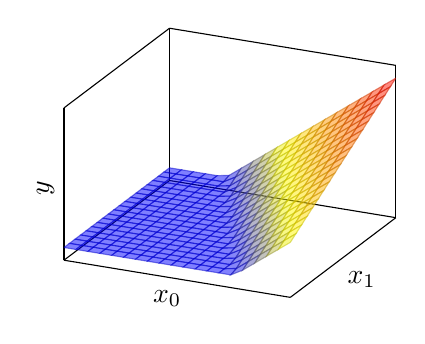
\begin{tikzpicture}[
				declare function = {
					q(\x) = \x - 1;
					Z(\x,\y) = max(0, \x*0.5 + \y*0.25);
				}
			]
				\begin{axis}
				[
					height=5cm,
					ticks=none,
					xlabel=$x_0$,
					ylabel=$x_1$,
					zlabel=$y$,
					domain=-1:1,
					samples=20,
				]
					\addplot3 [surf, opacity=0.5] {Z(x,y)};
				\end{axis}
			\end{tikzpicture}
		}
		\begin{tikzpicture}
			\node[] at (-5, 3) {};
			\node[] at (5, -4.5) {};

			\node[
				circle,
				draw=black,
				fill=green!20,
				minimum size=\nodesize,
				inner sep=0pt
			] (n) at (0, 1.5) {};
			\node[] (x0) at (-1.5, 2) {$x_0$};
			\node[] (x1) at (-1.5, 1) {$x_1$};
			\node[] (b) at (0, 2.5) {$b$};
			\node[] (y) at (1.5, 1.5) {$y$};
			\node[] at (0, 0) {$y=max(0, w_0x_0+w_1x_1+b)$};

			\draw[->] (x0) -- (n) node [midway, above] {$w_0$};
			\draw[->] (x1) -- (n) node [midway, below] {$w_1$};
			\draw[->] (b) -- (n);
			\draw[->] (n) -- (y);

			\node[] at (0, -2.75) {
				\usebox{\mybox}
			};
		\end{tikzpicture}
		\vfill
	\end{frame}

	\begin{frame}{Building a neural network}
		\centering
		\vfill
		\begin{tikzpicture}
			\node[] at (-3.5, 1.25) {};
			\node[] at (3.5, -6.25) {};
			\node[
				circle,
				minimum size=\nodesize,
				inner sep=0pt,
				text depth=0
			] (x) at (-3, 0) {\footnotesize{$x$}};

			\node[
				circle,
				draw=black,
				fill=green!20,
				minimum size=\nodesize,
				inner sep=0pt
			] (n00) at (0, 0.5) {};
			\node[
				circle,
				draw=black,
				fill=green!20,
				minimum size=\nodesize,
				inner sep=0pt
			] (n01) at (0, -0.5) {};

			\node[
				circle,
				minimum size=\nodesize,
				inner sep=0pt,
				text depth=0
			] (y) at (3, 0) {\footnotesize{$y$}};

			\draw[->] (x) -- (n00) node [midway, above] {$w_0$};
			\draw[->] (x) -- (n01) node [midway, below] {$w_1$};

			\draw[->] (n00) -- (y);
			\draw[->] (n01) -- (y);

			\def\spacing{-0.1cm}
			\node[anchor=north] at (0, -1.5) {\tiny{
				\begin{math}
					\begin{alignedat}{5}
						y = max(0, w_0x+b_0)+max(0, w_1x+b_1)\\
					\end{alignedat}
				\end{math}
			}};
		\end{tikzpicture}
		\vfill
	\end{frame}

	\begin{frame}{Building a neural network}
		\centering
		\vfill
		\begin{tikzpicture}
			\node[] at (-3.5, 1.25) {};
			\node[] at (3.5, -6.25) {};
			\node[
				circle,
				draw=black,
				fill=green!20,
				minimum size=\nodesize,
				inner sep=0pt,
				text depth=0
			] (x) at (-3, 0) {\footnotesize{$x$}};

			\node[
				circle,
				draw=black,
				fill=green!20,
				minimum size=\nodesize,
				inner sep=0pt
			] (n00) at (0, 0.5) {};
			\node[
				circle,
				draw=black,
				fill=green!20,
				minimum size=\nodesize,
				inner sep=0pt
			] (n01) at (0, -0.5) {};

			\node[
				circle,
				draw=black,
				fill=green!20,
				minimum size=\nodesize,
				inner sep=0pt,
				text depth=0
			] (y) at (3, 0) {\footnotesize{$y$}};

			\draw[->] (x) -- (n00) node [midway, above] {$w^0_0$};
			\draw[->] (x) -- (n01) node [midway, below] {$w^0_1$};

			\draw[->] (n00) -- (y) node [midway, above] {$w^1_0$};
			\draw[->] (n01) -- (y) node [midway, below] {$w^1_0$};

			\def\spacing{-0.1cm}
			\node[anchor=north] at (0, -1.5) {\tiny{
				\begin{math}
					\begin{alignedat}{5}
						y = max(0, w^1_{0,0}*max(0, w^0_{0,0}*x+b_{0,0})+w^1_{1,0}*max(0, w^0_{0,1}*x+b_{1,0})+b_1)\\
					\end{alignedat}
				\end{math}
			}};
		\end{tikzpicture}
		\vfill
	\end{frame}

	\begin{frame}{Building a neural network}
		\centering
		\vfill
		\begin{tikzpicture}
			\node[] at (-3.5, 1.25) {};
			\node[] at (3.5, -6.25) {};
			\node[
				circle,
				draw=black,
				fill=green!20,
				minimum size=\nodesize,
				inner sep=0pt,
				text depth=0
			] (x) at (-3, 0) {\footnotesize{$x$}};

			\node[
				circle,
				draw=black,
				fill=green!20,
				minimum size=\nodesize,
				inner sep=0pt
			] (n00) at (0, 0.5) {};
			\node[
				circle,
				draw=black,
				fill=green!20,
				minimum size=\nodesize,
				inner sep=0pt
			] (n01) at (0, -0.5) {};

			\node[
				circle,
				draw=black,
				fill=green!20,
				minimum size=\nodesize,
				inner sep=0pt,
				text depth=0
			] (y) at (3, 0) {\footnotesize{$y$}};

			\node[text depth=0] at (-3, -1.2) {\textcolor{red}{Input}};
			\node[text depth=0] at (0, -1.2) {\textcolor{red}{Hidden}};
			\node[text depth=0] at (3, -1.2) {\textcolor{red}{Output}};

			\draw[->] (x) -- (n00) node [midway, above] {$w^0_0$};
			\draw[->] (x) -- (n01) node [midway, below] {$w^0_1$};

			\draw[->] (n00) -- (y) node [midway, above] {$w^1_0$};
			\draw[->] (n01) -- (y) node [midway, below] {$w^1_0$};

			\def\spacing{-0.1cm}
			\node[anchor=north] at (0, -1.5) {\tiny{
				\begin{math}
					\begin{alignedat}{5}
						y = max(0, w^1_{0,0}*max(0, w^0_{0,0}*x+b_{0,0})+w^1_{1,0}*max(0, w^0_{0,1}*x+b_{1,0})+b_1)\\
					\end{alignedat}
				\end{math}
			}};
		\end{tikzpicture}
		\vfill
	\end{frame}

	\begin{frame}{Building a neural network}
		\centering
		\vfill
		\begin{tikzpicture}
			\node[] at (-3.5, 1.25) {};
			\node[] at (3.5, -6.25) {};
			\node[
				circle,
				draw=black,
				fill=green!20,
				minimum size=\nodesize,
				inner sep=0pt,
				text depth=0
			] (x0) at (-3, 0.5) {\footnotesize{$x_0$}};
			\node[
				circle,
				draw=black,
				fill=green!20,
				minimum size=\nodesize,
				inner sep=0pt,
				text depth=0
			] (x1) at (-3, -0.5) {\footnotesize{$x_1$}};

			\node[
				circle,
				draw=black,
				fill=green!20,
				minimum size=\nodesize,
				inner sep=0pt
			] (n00) at (0, 0.5) {};
			\node[
				circle,
				draw=black,
				fill=green!20,
				minimum size=\nodesize,
				inner sep=0pt
			] (n01) at (0, -0.5) {};

			\node[
				circle,
				draw=black,
				fill=green!20,
				minimum size=\nodesize,
				inner sep=0pt,
				text depth=0
			] (y) at (3, 0) {\footnotesize{$y$}};

			\draw[->] (x0) -- (n00);
			\draw[->] (x0) -- (n01);
			\draw[->] (x1) -- (n00);
			\draw[->] (x1) -- (n01);

			\draw[->] (n00) -- (y);
			\draw[->] (n01) -- (y);

			\def\spacing{-0.1cm}
			\node[anchor=north] at (0, -1.5) {\tiny{
				\begin{math}
					\begin{alignedat}{5}
						y &= max(0, &&w^1_{0,0}*max(0, w^0_{0,0}*x_0+w^0_{1,0}*x_{1}+b_{0,0})+\\[\spacing]
						& &&w^1_{1,0}*max(0, w^0_{0,1}*x_0+w^0_{1,1}*x_{1}+b_{0,1})+\\[\spacing]
						& &&b_1)&&\\
					\end{alignedat}
				\end{math}
			}};
		\end{tikzpicture}
		\vfill
	\end{frame}


	\begin{frame}{Building a neural network}
		\centering
		\vfill
		\begin{tikzpicture}
			\node[] at (-3.5, 1.25) {};
			\node[] at (3.5, -6.25) {};
			\node[
				circle,
				draw=black,
				fill=green!20,
				minimum size=\nodesize,
				inner sep=0pt,
				text depth=0
			] (x0) at (-3, 0.5) {\footnotesize{$x_0$}};
			\node[
				circle,
				draw=black,
				fill=green!20,
				minimum size=\nodesize,
				inner sep=0pt,
				text depth=0
			] (x1) at (-3, -0.5) {\footnotesize{$x_1$}};

			\node[
				circle,
				draw=black,
				fill=green!20,
				minimum size=\nodesize,
				inner sep=0pt
			] (n00) at (0, 1) {};
			\node[
				circle,
				draw=black,
				fill=green!20,
				minimum size=\nodesize,
				inner sep=0pt
			] (n01) at (0, 0) {};
			\node[
				circle,
				draw=black,
				fill=green!20,
				minimum size=\nodesize,
				inner sep=0pt
			] (n02) at (0, -1) {};

			\node[
				circle,
				draw=black,
				fill=green!20,
				minimum size=\nodesize,
				inner sep=0pt,
				text depth=0
			] (y) at (3, 0) {\footnotesize{$y$}};

			\draw[->] (x0) -- (n00);
			\draw[->] (x0) -- (n01);
			\draw[->] (x0) -- (n02);
			\draw[->] (x1) -- (n00);
			\draw[->] (x1) -- (n01);
			\draw[->] (x1) -- (n02);

			\draw[->] (n00) -- (y);
			\draw[->] (n01) -- (y);
			\draw[->] (n02) -- (y);

			\def\spacing{-0.1cm}
			\node[anchor=north] at (0, -1.5) {\tiny{
				\begin{math}
					\begin{alignedat}{5}
						y &= max(0, &&w^1_{0,0}*max(0, w^0_{0,0}*x_0+w^0_{1,0}*x_{1}+b_{0,0})+\\[\spacing]
						& &&w^1_{1,0}*max(0, w^0_{0,1}*x_0+w^0_{1,1}*x_{1}+b_{0,1})+\\[\spacing]
						& &&w^1_{2,0}*max(0, w^0_{0,2}*x_0+w^0_{1,2}*x_{1}+b_{0,2})+\\[\spacing]
						& &&b_1)&&\\
					\end{alignedat}
				\end{math}
			}};
		\end{tikzpicture}
		\vfill
	\end{frame}

	\begin{frame}{Building a neural network}
		\centering
		\vfill
		\begin{tikzpicture}
			\node[] at (-3.5, 1.25) {};
			\node[] at (3.5, -6.25) {};
			\node[
				circle,
				draw=black,
				fill=green!20,
				minimum size=\nodesize,
				inner sep=0pt,
				text depth=0
			] (x0) at (-3, 0.5) {\footnotesize{$x_0$}};
			\node[
				circle,
				draw=black,
				fill=green!20,
				minimum size=\nodesize,
				inner sep=0pt,
				text depth=0
			] (x1) at (-3, -0.5) {\footnotesize{$x_1$}};

			\node[
				circle,
				draw=black,
				fill=green!20,
				minimum size=\nodesize,
				inner sep=0pt
			] (n00) at (-1, 1) {};
			\node[
				circle,
				draw=black,
				fill=green!20,
				minimum size=\nodesize,
				inner sep=0pt
			] (n01) at (-1, 0) {};
			\node[
				circle,
				draw=black,
				fill=green!20,
				minimum size=\nodesize,
				inner sep=0pt
			] (n02) at (-1, -1) {};

			\node[
				circle,
				draw=black,
				fill=green!20,
				minimum size=\nodesize,
				inner sep=0pt
			] (n10) at (1, 1) {};

			\node[
				circle,
				draw=black,
				fill=green!20,
				minimum size=\nodesize,
				inner sep=0pt
			] (n11) at (1, 0) {};
			\node[
				circle,
				draw=black,
				fill=green!20,
				minimum size=\nodesize,
				inner sep=0pt
			] (n12) at (1, -1) {};

			\node[
				circle,
				draw=black,
				fill=green!20,
				minimum size=\nodesize,
				inner sep=0pt,
				text depth=0
			] (y) at (3, 0) {\footnotesize{$y$}};

			\draw[->] (x0) -- (n00);
			\draw[->] (x0) -- (n01);
			\draw[->] (x0) -- (n02);
			\draw[->] (x1) -- (n00);
			\draw[->] (x1) -- (n01);
			\draw[->] (x1) -- (n02);

			\draw[->] (n00) -- (n10);
			\draw[->] (n00) -- (n11);
			\draw[->] (n00) -- (n12);
			\draw[->] (n01) -- (n10);
			\draw[->] (n01) -- (n11);
			\draw[->] (n01) -- (n12);
			\draw[->] (n02) -- (n10);
			\draw[->] (n02) -- (n11);
			\draw[->] (n02) -- (n12);

			\draw[->] (n10) -- (y);
			\draw[->] (n11) -- (y);
			\draw[->] (n12) -- (y);

			\def\spacing{-0.1cm}
			\node[anchor=north] at (0, -1.5) {\tiny{
				\begin{math}
					\begin{alignedat}{5}
						y &= max(0, &&w^2_{0,0}*max(0, &&w^1_{0,0}*max(0, w^0_{0,0}*x_0+w^0_{1,0}*x_{1}+b_{0,0})+\\[\spacing]
						& && &&w^1_{1,0}*max(0, w^0_{0,1}*x_0+w^+_{1,1}*w_{1}+b_{0,1})+\\[\spacing]
						& && &&w^1_{2,0}*max(0, w^0_{0,2}*x_0+w^+_{1,2}*w_{1}+b_{0,2})+\\[\spacing]
						& && &&b_{1,0})+\\[\spacing]
						& &&w^2_{1,0}*max(0, &&w^1_{0,1}*max(0, w^0_{0,0}*x_0+w^0_{1,0}*x_{1}+b_{0,0})+\\[\spacing]
						& && &&w^1_{1,1}*max(0, w^0_{0,1}*x_0+w^+_{1,1}*w_{1}+b_{0,1})+\\[\spacing]
						& && &&w^1_{2,1}*max(0, w^0_{0,2}*x_0+w^+_{1,2}*w_{1}+b_{0,2})+\\[\spacing]
						& && &&b_{1,1})+\\[\spacing]
						& &&w^2_{2,0}*max(0, &&w^1_{0,2}*max(0, w^0_{0,0}*x_0+w^0_{1,0}*x_{1}+b_{0,0})+\\[\spacing]
						& && &&w^1_{1,2}*max(0, w^0_{0,1}*x_0+w^+_{1,1}*w_{1}+b_{0,1})+\\[\spacing]
						& && &&w^1_{2,2}*max(0, w^0_{0,2}*x_0+w^+_{1,2}*w_{1}+b_{0,2})+\\[\spacing]
						& && &&b_{1,2})+\\[\spacing]
						& &&b_2)&&\\
					\end{alignedat}
				\end{math}
			}};
		\end{tikzpicture}
		\vfill
	\end{frame}

	\begin{frame}{Building a neural network: Summary}
		\centering
		\vfill
		\begin{itemize}
			\item Artificial neurons are (linear) weighted sums wrapped in non-linear activation functions
			\item Multiple artificial neurons stacked together in a layerwise fashion comprise an artificial neural network
			\item Artificial neural networks allow us to model arbitrarily complex relationships between inputs and outputs
		\end{itemize}
		\vfill
	\end{frame}
\end{document}
